\documentclass[border=6pt]{standalone}
\usepackage{tikz}
\begin{document}
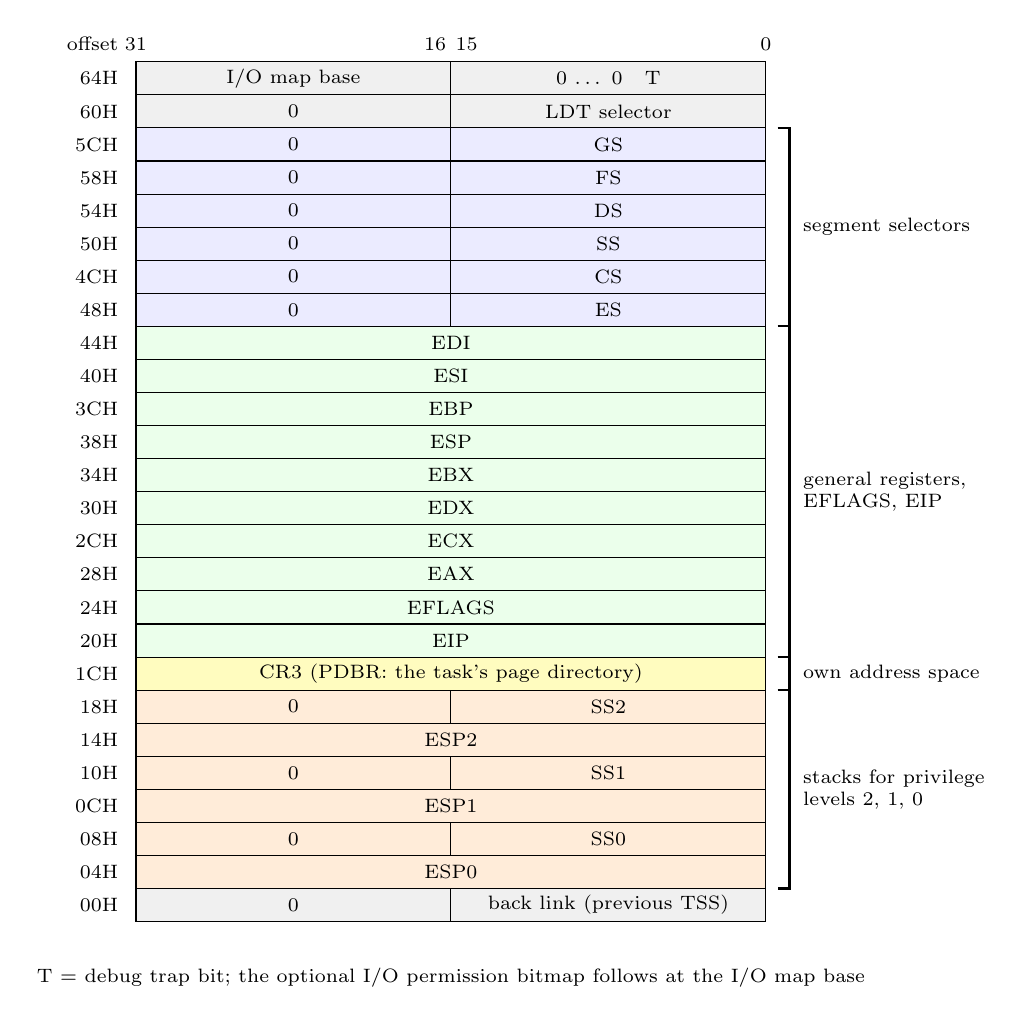
\begin{tikzpicture}[font=\small,x=1cm,y=0.42cm]
\node[font=\scriptsize,anchor=south] at (0,0.05) {31};\node[font=\scriptsize,anchor=south] at (3.8,0.05) {16};\node[font=\scriptsize,anchor=south] at (4.2,0.05) {15};\node[font=\scriptsize,anchor=south] at (8,0.05) {0};
\node[font=\scriptsize,anchor=south east] at (-0.1,0.05) {offset};
\node[font=\scriptsize,anchor=east] at (-0.1,-0.5) {64H};
\draw[fill=gray!12] (0,-1) rectangle (4,0); \node[font=\scriptsize] at (2,-0.5) {I/O map base};
\draw[fill=gray!12] (4,-1) rectangle (8,0); \node[font=\scriptsize] at (6,-0.5) {0 \dots\ 0\quad T};
\node[font=\scriptsize,anchor=east] at (-0.1,-1.5) {60H};
\draw[fill=gray!12] (0,-2) rectangle (4,-1); \node[font=\scriptsize] at (2,-1.5) {0};
\draw[fill=gray!12] (4,-2) rectangle (8,-1); \node[font=\scriptsize] at (6,-1.5) {LDT selector};
\node[font=\scriptsize,anchor=east] at (-0.1,-2.5) {5CH};
\draw[fill=blue!8] (0,-3) rectangle (4,-2); \node[font=\scriptsize] at (2,-2.5) {0};
\draw[fill=blue!8] (4,-3) rectangle (8,-2); \node[font=\scriptsize] at (6,-2.5) {GS};
\node[font=\scriptsize,anchor=east] at (-0.1,-3.5) {58H};
\draw[fill=blue!8] (0,-4) rectangle (4,-3); \node[font=\scriptsize] at (2,-3.5) {0};
\draw[fill=blue!8] (4,-4) rectangle (8,-3); \node[font=\scriptsize] at (6,-3.5) {FS};
\node[font=\scriptsize,anchor=east] at (-0.1,-4.5) {54H};
\draw[fill=blue!8] (0,-5) rectangle (4,-4); \node[font=\scriptsize] at (2,-4.5) {0};
\draw[fill=blue!8] (4,-5) rectangle (8,-4); \node[font=\scriptsize] at (6,-4.5) {DS};
\node[font=\scriptsize,anchor=east] at (-0.1,-5.5) {50H};
\draw[fill=blue!8] (0,-6) rectangle (4,-5); \node[font=\scriptsize] at (2,-5.5) {0};
\draw[fill=blue!8] (4,-6) rectangle (8,-5); \node[font=\scriptsize] at (6,-5.5) {SS};
\node[font=\scriptsize,anchor=east] at (-0.1,-6.5) {4CH};
\draw[fill=blue!8] (0,-7) rectangle (4,-6); \node[font=\scriptsize] at (2,-6.5) {0};
\draw[fill=blue!8] (4,-7) rectangle (8,-6); \node[font=\scriptsize] at (6,-6.5) {CS};
\node[font=\scriptsize,anchor=east] at (-0.1,-7.5) {48H};
\draw[fill=blue!8] (0,-8) rectangle (4,-7); \node[font=\scriptsize] at (2,-7.5) {0};
\draw[fill=blue!8] (4,-8) rectangle (8,-7); \node[font=\scriptsize] at (6,-7.5) {ES};
\node[font=\scriptsize,anchor=east] at (-0.1,-8.5) {44H};
\draw[fill=green!8] (0,-9) rectangle (8,-8); \node[font=\scriptsize] at (4,-8.5) {EDI};
\node[font=\scriptsize,anchor=east] at (-0.1,-9.5) {40H};
\draw[fill=green!8] (0,-10) rectangle (8,-9); \node[font=\scriptsize] at (4,-9.5) {ESI};
\node[font=\scriptsize,anchor=east] at (-0.1,-10.5) {3CH};
\draw[fill=green!8] (0,-11) rectangle (8,-10); \node[font=\scriptsize] at (4,-10.5) {EBP};
\node[font=\scriptsize,anchor=east] at (-0.1,-11.5) {38H};
\draw[fill=green!8] (0,-12) rectangle (8,-11); \node[font=\scriptsize] at (4,-11.5) {ESP};
\node[font=\scriptsize,anchor=east] at (-0.1,-12.5) {34H};
\draw[fill=green!8] (0,-13) rectangle (8,-12); \node[font=\scriptsize] at (4,-12.5) {EBX};
\node[font=\scriptsize,anchor=east] at (-0.1,-13.5) {30H};
\draw[fill=green!8] (0,-14) rectangle (8,-13); \node[font=\scriptsize] at (4,-13.5) {EDX};
\node[font=\scriptsize,anchor=east] at (-0.1,-14.5) {2CH};
\draw[fill=green!8] (0,-15) rectangle (8,-14); \node[font=\scriptsize] at (4,-14.5) {ECX};
\node[font=\scriptsize,anchor=east] at (-0.1,-15.5) {28H};
\draw[fill=green!8] (0,-16) rectangle (8,-15); \node[font=\scriptsize] at (4,-15.5) {EAX};
\node[font=\scriptsize,anchor=east] at (-0.1,-16.5) {24H};
\draw[fill=green!8] (0,-17) rectangle (8,-16); \node[font=\scriptsize] at (4,-16.5) {EFLAGS};
\node[font=\scriptsize,anchor=east] at (-0.1,-17.5) {20H};
\draw[fill=green!8] (0,-18) rectangle (8,-17); \node[font=\scriptsize] at (4,-17.5) {EIP};
\node[font=\scriptsize,anchor=east] at (-0.1,-18.5) {1CH};
\draw[fill=yellow!25] (0,-19) rectangle (8,-18); \node[font=\scriptsize] at (4,-18.5) {CR3 (PDBR: the task's page directory)};
\node[font=\scriptsize,anchor=east] at (-0.1,-19.5) {18H};
\draw[fill=orange!15] (0,-20) rectangle (4,-19); \node[font=\scriptsize] at (2,-19.5) {0};
\draw[fill=orange!15] (4,-20) rectangle (8,-19); \node[font=\scriptsize] at (6,-19.5) {SS2};
\node[font=\scriptsize,anchor=east] at (-0.1,-20.5) {14H};
\draw[fill=orange!15] (0,-21) rectangle (8,-20); \node[font=\scriptsize] at (4,-20.5) {ESP2};
\node[font=\scriptsize,anchor=east] at (-0.1,-21.5) {10H};
\draw[fill=orange!15] (0,-22) rectangle (4,-21); \node[font=\scriptsize] at (2,-21.5) {0};
\draw[fill=orange!15] (4,-22) rectangle (8,-21); \node[font=\scriptsize] at (6,-21.5) {SS1};
\node[font=\scriptsize,anchor=east] at (-0.1,-22.5) {0CH};
\draw[fill=orange!15] (0,-23) rectangle (8,-22); \node[font=\scriptsize] at (4,-22.5) {ESP1};
\node[font=\scriptsize,anchor=east] at (-0.1,-23.5) {08H};
\draw[fill=orange!15] (0,-24) rectangle (4,-23); \node[font=\scriptsize] at (2,-23.5) {0};
\draw[fill=orange!15] (4,-24) rectangle (8,-23); \node[font=\scriptsize] at (6,-23.5) {SS0};
\node[font=\scriptsize,anchor=east] at (-0.1,-24.5) {04H};
\draw[fill=orange!15] (0,-25) rectangle (8,-24); \node[font=\scriptsize] at (4,-24.5) {ESP0};
\node[font=\scriptsize,anchor=east] at (-0.1,-25.5) {00H};
\draw[fill=gray!12] (0,-26) rectangle (4,-25); \node[font=\scriptsize] at (2,-25.5) {0};
\draw[fill=gray!12] (4,-26) rectangle (8,-25); \node[font=\scriptsize] at (6,-25.5) {back link (previous TSS)};
\draw[thick] (8.15,-2) -- (8.3,-2) -- (8.3,-8) -- (8.15,-8);
\node[font=\scriptsize,anchor=west,align=left] at (8.35,-5) {segment selectors};
\draw[thick] (8.15,-8) -- (8.3,-8) -- (8.3,-18) -- (8.15,-18);
\node[font=\scriptsize,anchor=west,align=left] at (8.35,-13) {general registers,\\EFLAGS, EIP};
\draw[thick] (8.15,-18) -- (8.3,-18) -- (8.3,-19) -- (8.15,-19);
\node[font=\scriptsize,anchor=west,align=left] at (8.35,-18.5) {own address space};
\draw[thick] (8.15,-19) -- (8.3,-19) -- (8.3,-25) -- (8.15,-25);
\node[font=\scriptsize,anchor=west,align=left] at (8.35,-22) {stacks for privilege\\levels 2, 1, 0};
\node[font=\scriptsize,anchor=north] at (4,-27.1) {T = debug trap bit; the optional I/O permission bitmap follows at the I/O map base};
\end{tikzpicture}
\end{document}
